\documentclass[
  bibliography=totoc,     % Literatur im Inhaltsverzeichnis
  captions=tableheading,  % Tabellenüberschriften
  titlepage=firstiscover, % Titelseite ist Deckblatt
]{scrartcl}

% Paket float verbessern
\usepackage{scrhack}

% Warnung, falls nochmal kompiliert werden muss
\usepackage[aux]{rerunfilecheck}

% unverzichtbare Mathe-Befehle
\usepackage{amsmath}
% viele Mathe-Symbole
\usepackage{amssymb}
% Erweiterungen für amsmath
\usepackage{mathtools}

% Fonteinstellungen
\usepackage{fontspec}
% Latin Modern Fonts werden automatisch geladen
% Alternativ:
%\setromanfont{Libertinus Serif}
%\setsansfont{Libertinus Sans}
%\setmonofont{Libertinus Mono}
\recalctypearea % Wenn man andere Schriftarten gesetzt hat,
% sollte man das Seiten-Layout neu berechnen lassen

% deutsche Spracheinstellungen
\usepackage{polyglossia}
\setmainlanguage{german}


\usepackage[
  math-style=ISO,    % ┐
  bold-style=ISO,    % │
  sans-style=italic, % │ ISO-Standard folgen
  nabla=upright,     % │
  partial=upright,   % ┘
  warnings-off={           % ┐
    mathtools-colon,       % │ unnötige Warnungen ausschalten
    mathtools-overbracket, % │
},                       % ┘
]{unicode-math}

% traditionelle Fonts für Mathematik
\setmathfont{Latin Modern Math}
% Alternativ:
%\setmathfont{Libertinus Math}

\setmathfont{XITS Math}[range={scr, bfscr}]
\setmathfont{XITS Math}[range={cal, bfcal}, StylisticSet=1]

% Zahlen und Einheiten
\usepackage[
locale=DE,                   % deutsche Einstellungen
separate-uncertainty=true,   % immer Fehler mit \pm
per-mode=symbol-or-fraction, % / in inline math, fraction in display math
]{siunitx}

% chemische Formeln
\usepackage[
version=4,
math-greek=default, % ┐ mit unicode-math zusammenarbeiten
text-greek=default, % ┘
]{mhchem}

% richtige Anführungszeichen
\usepackage[autostyle]{csquotes}

% schöne Brüche im Text
\usepackage{xfrac}

% Standardplatzierung für Floats einstellen
\usepackage{float}
\floatplacement{figure}{htbp}
\floatplacement{table}{htbp}

% Floats innerhalb einer Section halten
\usepackage[
section, % Floats innerhalb der Section halten
below,   % unterhalb der Section aber auf der selben Seite ist ok
]{placeins}

% Seite drehen für breite Tabellen: landscape Umgebung
\usepackage{pdflscape}

% Captions schöner machen.
\usepackage[
  labelfont=bf,        % Tabelle x: Abbildung y: ist jetzt fett
  font=small,          % Schrift etwas kleiner als Dokument
  width=0.9\textwidth, % maximale Breite einer Caption schmaler
]{caption}
% subfigure, subtable, subref
\usepackage{subcaption}

% Grafiken können eingebunden werden
\usepackage{graphicx}
% größere Variation von Dateinamen möglich
\usepackage{grffile}

% schöne Tabellen
\usepackage{booktabs}

% Verbesserungen am Schriftbild
\usepackage{microtype}

% Literaturverzeichnis
\usepackage[style=alphabetic,]{biblatex}
% Quellendatenbank
\addbibresource{lit.bib}

% Hyperlinks im Dokument
\usepackage[
  unicode,        % Unicode in PDF-Attributen erlauben
  pdfusetitle,    % Titel, Autoren und Datum als PDF-Attribute
  pdfcreator={},  % ┐ PDF-Attribute säubern
  pdfproducer={}, % ┘
]{hyperref}
% erweiterte Bookmarks im PDF
\usepackage{bookmark}

% Trennung von Wörtern mit Strichen
\usepackage[shortcuts]{extdash}

\title{V406: Beugung am Spalt}
\author{
  Simon Schulte
  \texorpdfstring{
    \\
    \href{mailto:simon.schulte@udo.edu}{simon.schulte@udo.edu}
  }{}
  \texorpdfstring{\and}{, }
  Tim Sedlaczek
  \texorpdfstring{
    \\
    \href{mailto:tim.sedlaczek@udo.edu}{tim.sedlaczek@udo.edu}
  }{}
}
\publishers{TU Dortmund – Fakultät Physik}

\date{Durchführung: 09.05.2017\\
      Abgabe: 16.05.2017}


\begin{document}

\maketitle
\thispagestyle{empty}
\tableofcontents
\newpage
\setcounter{page}{1}
\section{Zielsetzung}
\label{sec:zielsetzung}
Ziel des Versuchs ist die Untersuchung von Lichtbeugung an einem Einzelspalt und zwei Doppelspalten.
\section{Theorie}
\label{sec:theorie}
Die Beugung des Lichts beschreibt die Abweichung der Lichtausbreitung von den
Gesetzen der geometrischen Optik. Nach dem Huygensschen Prinzip und dem Interferenzprinzip von Fresnel werden von jedem Punkt einer Wellenfläche Elementarwellen ausgesendet. Diese breiten sich kugelwellenartig aus. Dabei interferieren sie miteinander.
\begin{figure}[htb]
  \centering
  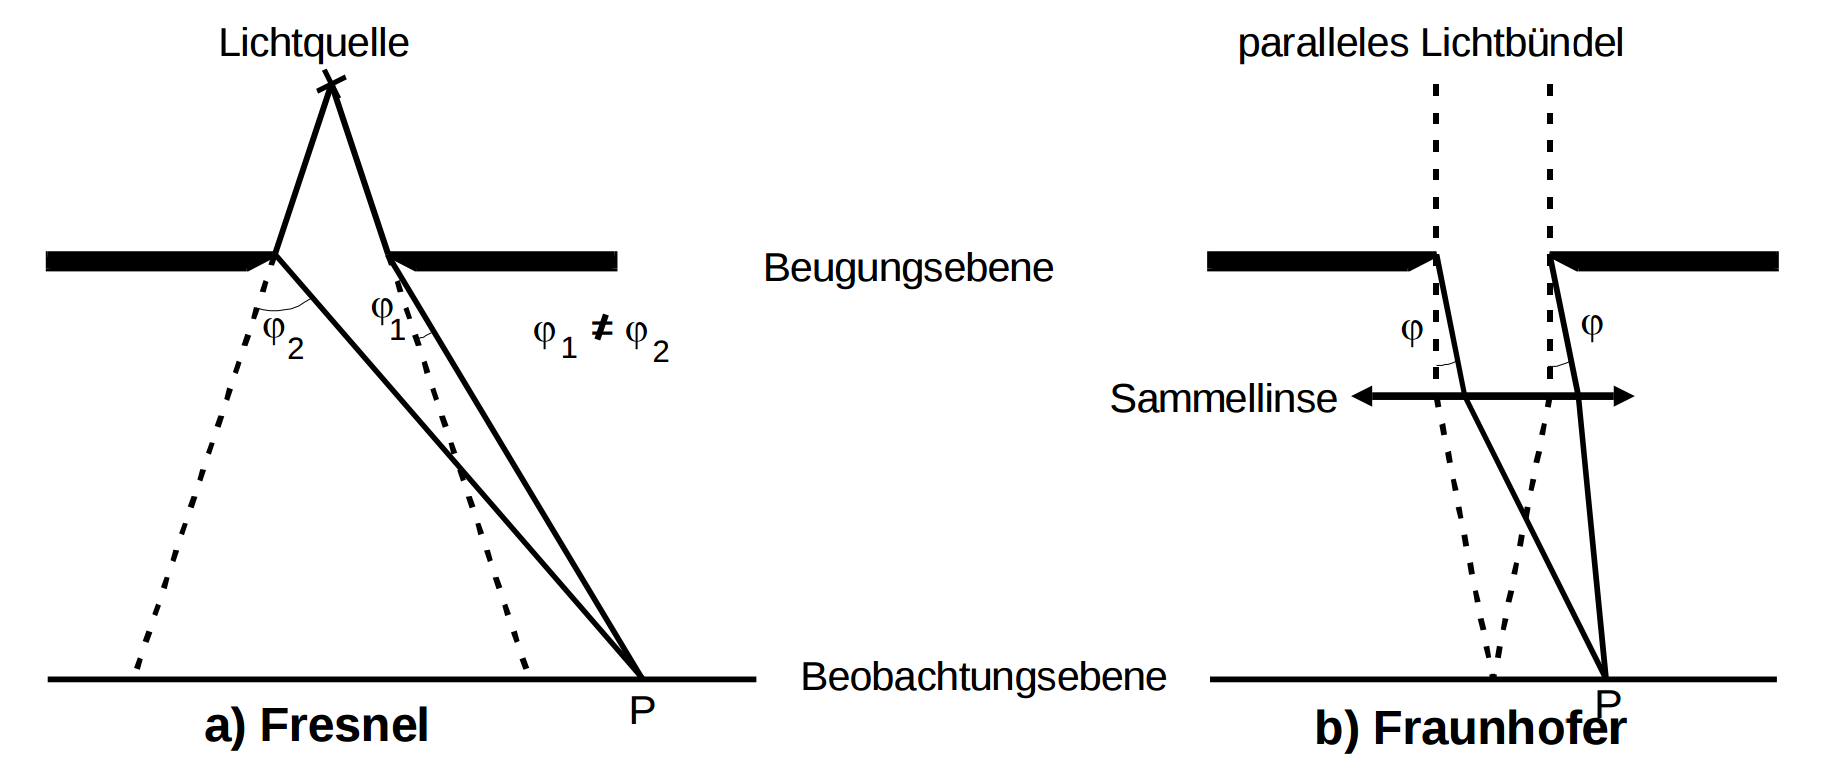
\includegraphics[width=0.9\textwidth]{V4061.png}
  \caption{Die Fesnelsche und Franhofersche Beugung an einem Einfachspalt. \cite{anleitung}}
  \label{fig:V4061}
\end{figure}
Abbildung \ref{fig:V4061} zeigt die Fresnelsche und Fraunhofersche Beugung an einem Einzelspalt. In diesem Versuch wird lediglich die Fraunhofersche Beugung betrachtet, da diese mathematisch einfacher zu beschreiben ist. Hierbei wird von einem parallel ankommenden Strahl ausgegangen. Die getrichelten Linien stellen den Verlauf der geometrischen Optik dar. Bei der Fraunhoferschen Beugung werden die Lichtstrahlen aber teilweise um den Winkel $\phi$ gebeugt. Dadurch interferieren sie im Punkt $P$. Um nun die Amplitude eines Einzelspalts zu bestimmen, muss über alle Strahlenbündel, welche um den Winkel $\phi$ ausgelenkt werden, summiert werden. Eine hier betrachtete Welle wird durch
\begin{equation}
  A(z,t)\,=\,A_0\exp\Big(i\Big(\omega t-2\pi \frac{z}{\lambda}\Big)\Big)
  \label{eqn:welle}
\end{equation}
beschrieben. Diese hat den Phasenunterschied:
\begin{equation}
  \delta\,=\,\frac{2\pi x\sin(\phi)}{\lambda}.
  \label{eqn:phasenunterschied}
\end{equation}
In Abbildung \ref{fig:V4065} wird genau dies skizziert.
\begin{figure}[htb]
  \centering
  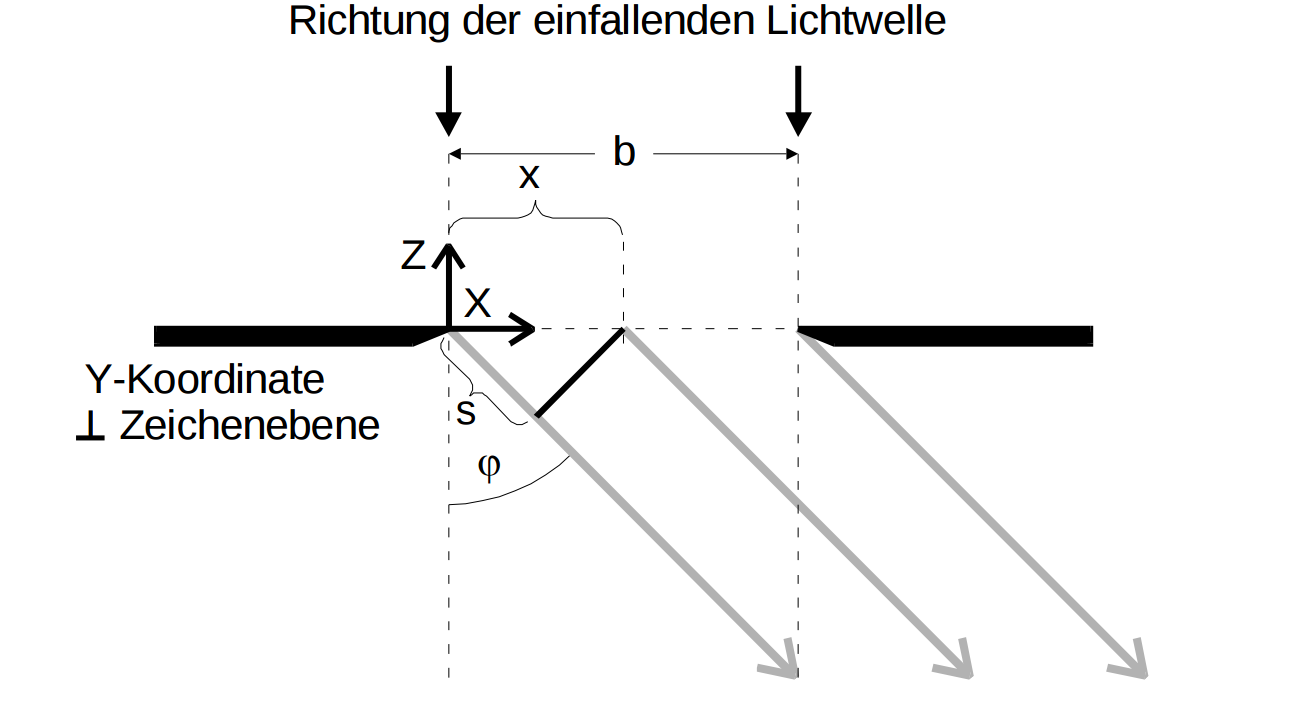
\includegraphics[width=0.9\textwidth]{V4065.png}
  \caption{Eine Skizze zur Ableitung einer Phasenbeziehung zwischen 2 Teilstrahlen bei der Fraunhoferschen Beugung am Spalt. \cite{anleitung}}
  \label{fig:V4065}
\end{figure}
Die Strahlenbündel vom Laser sind sehr klein. Daher wird über die Spaltbreite $D$ integriert. Da sich die Amplitude nicht direkt messen lässt, weil nicht nur ein einzelnes Photon betrachtet wird, sondern eine Intensität, wird zur Überprüfung ebenfalls die zeitlich gemittelte Intensität $I(\phi)$ bestimmt. Dabei ergibt sich folgender Zusammenhang:
\begin{equation}
  I(\phi)\,\propto\,B(\phi)²\,=\,A_0 b²\Big(\frac{\lambda}{\pi b\sin(\phi)}\Big)²\cdot \sin²\Big(\frac{\pi b\sin(\phi)}{\lambda}\Big).
  \label{eqn:intensitätsverteilungeinzel}
\end{equation}
Ein Doppelspalt kann physikalisch auch als Überlagerung zweier Einzelspalte gesehen werden. Abbildung \ref{fig:V4064} zeigt eine Beugung am Doppelspalt, an der dies gut erkennbar ist. Dann ergibt sich für die Intensitätsverteilung eines Doppelspalts
\begin{equation}
  I(\phi)\,\propto\,B(\phi)²\,=\,A_0\cos²\Big(\frac{\pi s\sin(\phi)}{\lambda}\Big)\cdot\Big(\frac{\lambda}{\pi b\sin(\phi)}\Big)²\cdot \sin²\Big(\frac{\pi b\sin(\phi)}{\lambda}\Big).
  \label{eqn:intensitätsverteilungdoppel}
\end{equation}
\begin{figure}[htb]
  \centering
  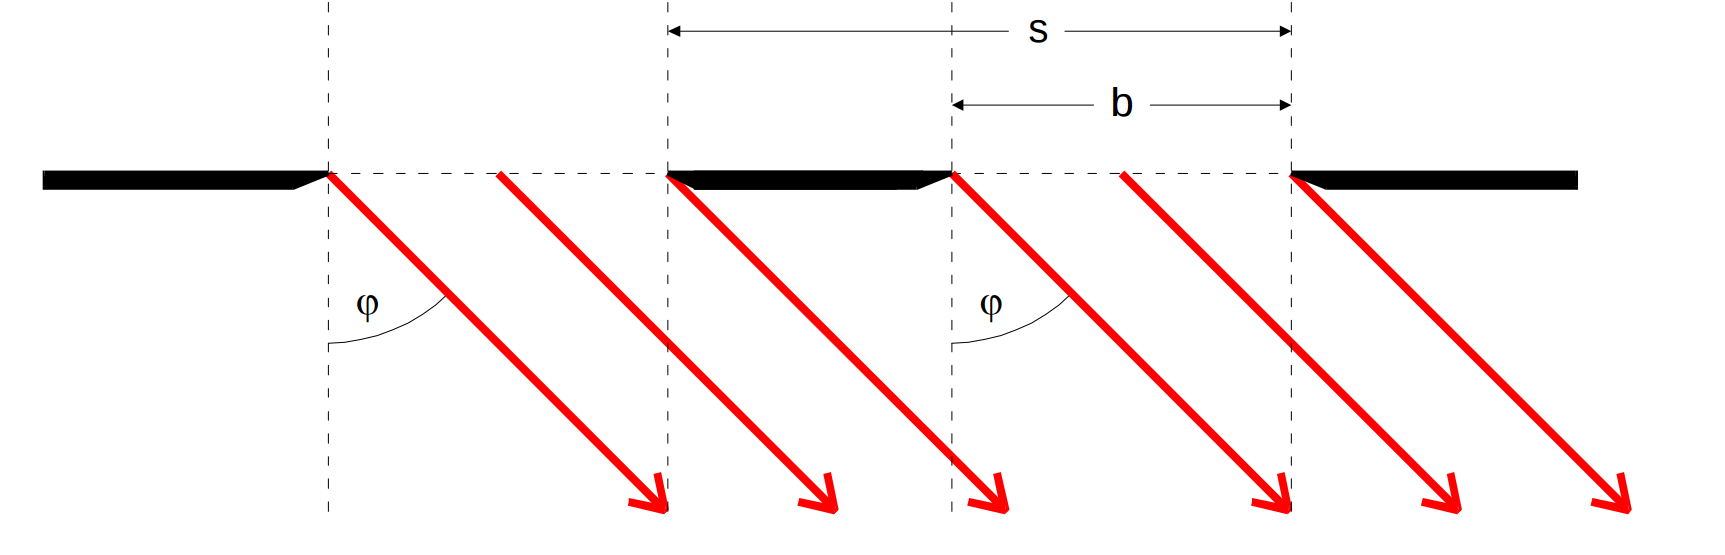
\includegraphics[width=0.9\textwidth]{V4064.png}
  \caption{Die Beugung am Doppelspalt. \cite{anleitung}}
  \label{fig:V4064}
\end{figure}

\section{Durchführung}
\subsection{Versuchsaufbau}
\label{sec:Versuchsaufbau}
\begin{figure}[htb]
  \centering
  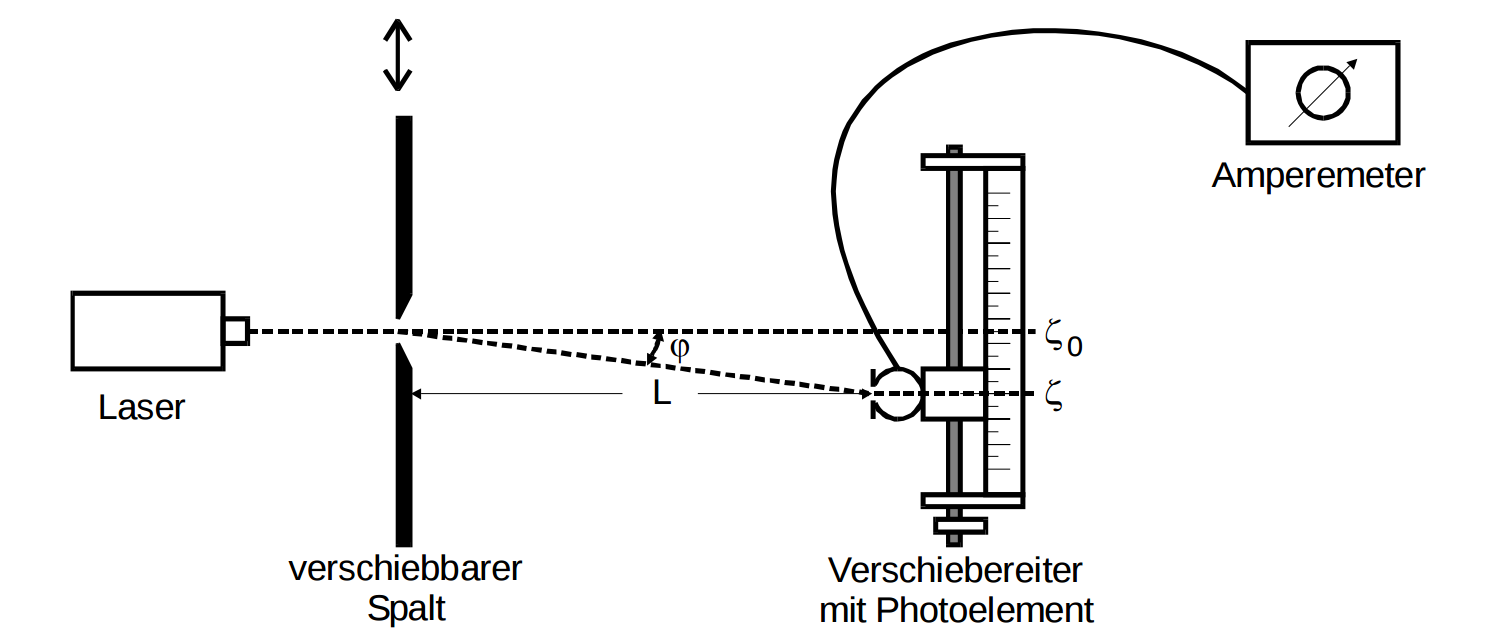
\includegraphics[width=0.9\textwidth]{V4063.png}
  \caption{Der Versuchsaufbau zur Ausmessung einer Beugungsfigur. \cite{anleitung}}
  \label{fig:V4063}
\end{figure}
In Abbildung \ref{fig:V4063} zu sehen ist der in dem Versuch verwendete Versuchsaufbau. Ein Laser sendet Lichtwellen mit einer Wellenlänge von \SI{635}{\nano\metre} aus. Dies ist notwendig, da Lichtbeugung nur auftritt, wenn der Spalt, an dem es gebeugt wird, ungefähr der Größenordnung der Wellenlänge $\lambda$ entspricht. Die Lichtwellen laufen durch einen Spalt, welcher in dem Versuch drei mal variiert wird. Dann kommen die Lichtwellen nach einer Strecke von L=\SI{124}{\centi\metre} an einem Verschiebereiter mit Photoelement an. Dieser misst die Intensität der einlaufenden Welle und schickt die Information an ein Amperemeter, an welchem dann der Diodenstrom ablesen werden kann.
\clearpage
\subsection{Versuchsablauf}
\label{sec:Versuchsablauf}
Als erstes werden die Spaltbreiten $b$ und die Gitterkonstanten $s$, der jeweils verwendeten Spalten, den Herstellerangeben entnommen.
Die Spaltbreite $b_E$ beträgt für den Einfachspalt
\begin{equation*}
  b_\mathup{E}\,=\,\SI{0.075}{\milli\metre}.
\end{equation*}
Für den ersten verwendeten Doppelspalt sind
\begin{align*}
  b_\mathup{D1} &= \SI{0.1}{\milli\metre}\\
  s_\mathup{D1} &= \SI{0.4}{\milli\metre}
\end{align*}
angegeben.

\noindent
Für den zweiten verwendeten Doppelspalt sind
\begin{align*}
  b_\mathup{D2} &= \SI{0.15}{\milli\metre}\\
  s_\mathup{D2} &= \SI{0.25}{\milli\metre}
\end{align*}
angegeben.

\noindent
Danach wird gemessen, was für einen Diodenstrom das Amperemeter registriert, wenn der Laser noch nicht eingeschaltet ist. Dies wird Dunkelmessung gennant und dieser Wert wird dann von den anderen Werten abgezogen, da die Lichtwellen, die sich im Raum befinden und auf das Amperemeter treffen die Messung verfälschen.
Die Dunkelmessung $d1$ ergibt einen Wert von
\begin{equation*}
  A_{d1}\,=\,\SI{1.15}{\nano\ampere}.
\end{equation*}
Zwischen den Messungen, für den Einzelspalt und den ersten Doppelspalt, wird die Dunkelmessung $d2$ wiederholt.
Dabei ergibt sich ein Wert von
\begin{equation*}
  A_{d2}\,=\,\SI{1.25}{\nano\ampere}.
\end{equation*}
Danach werden 93 Werte im Bereich von \SI{1}{\milli\metre} bis \SI{50}{\milli\metre} am Verschiebereiter mit Photoelement für den Diodenstrom aufgenommen. Dazu wird ein Einfachspalt verwendet.
Als nächstes werden 56 Werte zwischen \SI{14.25}{\milli\metre} und \SI{40.25}{\milli\metre} für den Diodenstrom aufgenommen. Dazu wird der erste Doppelspalt verwendet.
Als letztes werden 50 Werte im Bereich von \SI{11.25}{\milli\metre} bis \SI{40.75}{\milli\metre} für den Diodenstrom aufgenommen. Dazu wird der zweite Doppelspalt verwendet.
\clearpage
\section{Auswertung}
\label{sec:auswertung}
\subsection{Intensitätsverteilung am Einzelspalt}
Bei der Messung am Einzelspalt werden die in Tabelle \ref{tab:messwerte1}
stehenden Werte gemessen. Von diesen Werten wird zuerst der Dunkelstrom
$A_{d1}$ abgezogen und dann mit der Funktion curve-fit von Python eine
Kurvenanpassung an Formel \eqref{eqn:intensitätsverteilungeinzel} durchgeführt.
Die Wellenlänge des Lasers ist dabei mit
\begin{equation*}
  \lambda = \SI{635}{\nano\meter}
\end{equation*}
angegeben. Für $\phi$ wird näherungsweise
\begin{equation}
  \phi = \frac{x-x_0}{L}
\end{equation}
angenommen. Wobei $x_0$ die Position des Hauptmaximums darstellt. Während L
der Abstand zwischen Spalt und Photodiode ist. Dieser beträgt in unserem Fall
\begin{equation*}
  L = \SI{124}{\centi\meter}.
\end{equation*}
Die freien drei Parameter $A_0$, $b$ und $x_0$ werden also bei dem Fit
bestimmt:
\begin{align*}
  A_0 &= \SI{170(1)}{}\\
  b &= \SI{75.7(3)}{\micro\meter}\\
  x_0 &= \SI{26.38(2)}{\milli\meter}
\end{align*}
In Abbildung \ref{fig:plot1} ist der Verlauf der Messwerte, sowie des Fits,
zu sehen.
\begin{table}
  \centering
  \caption{Gemessener Diodenstrom bei der jeweiligen Position der Photodiode (ohne Abzug des Dunkelstroms).}
  \label{tab:messwerte1}
  \sisetup{table-format=2.2}
  \begin{tabular}{S S[table-format=3.0] | S S[table-format=3.0] | S S[table-format=3.0]}
    \toprule
     {$x$ in $\si{\milli\meter}$} & {$I$ in $\si{\nano\ampere}$} & {$x$} & {$I$} & {$x$} & {$I$} \\
    \midrule
    26.25 & 990 & 38.00 &  38 & 21.00 & 360 \\
    27.25 & 980 & 38.50 &  45 & 20.75 & 330 \\
    27.50 & 960 & 39.00 &  52 & 20.25 & 300 \\
    27.75 & 930 & 40.00 &  60 & 20.00 & 240 \\
    28.00 & 900 & 41.00 &  60 & 19.50 & 180 \\
    28.50 & 850 & 42.00 &  53 & 19.00 & 140 \\
    28.75 & 820 & 42.50 &  47 & 18.50 & 100 \\
    29.00 & 790 & 43.00 &  40 & 18.25 &  85 \\
    29.25 & 760 & 44.00 &  27 & 18.00 &  71 \\
    29.50 & 710 & 45.00 &  16 & 17.50 &  52 \\
    29.75 & 680 & 46.00 &  10 & 17.25 &  44 \\
    30.00 & 640 & 47.00 &  10 & 16.75 &  36 \\
    30.25 & 600 & 49.00 &  18 & 16.00 &  32 \\
    30.50 & 560 & 49.50 &  20 & 15.00 &  40 \\
    30.75 & 520 & 50.00 &  22 & 14.50 &  46 \\
    31.00 & 480 & 25.25 & 940 & 14.00 &  52 \\
    31.25 & 440 & 25.00 & 920 & 13.50 &  57 \\
    31.50 & 400 & 24.75 & 900 & 12.50 &  62 \\
    31.75 & 360 & 24.50 & 870 & 11.50 &  59 \\
    32.25 & 300 & 24.00 & 810 & 10.50 &  49 \\
    32.50 & 260 & 23.75 & 790 & 10.00 &  42 \\
    33.00 & 200 & 23.50 & 740 &  9.50 &  35 \\
    33.50 & 150 & 23.25 & 710 &  8.50 &  22 \\
    34.00 & 110 & 23.00 & 670 &  7.50 &  12 \\
    34.25 & 100 & 22.75 & 640 &  6.50 &   8 \\
    34.50 &  80 & 22.50 & 600 &  5.50 &  10 \\
    35.00 &  56 & 22.25 & 560 &  3.50 &  19 \\
    35.25 &  47 & 22.00 & 520 &  3.00 &  21 \\
    35.75 &  34 & 21.75 & 480 &  2.50 &  22 \\
    36.50 &  26 & 21.50 & 440 &  2.00 &  23 \\
    37.50 &  32 & 21.25 & 400 &  1.00 &  21 \\
    \bottomrule
  \end{tabular}
\end{table}
\clearpage
\begin{figure}
  \centering
  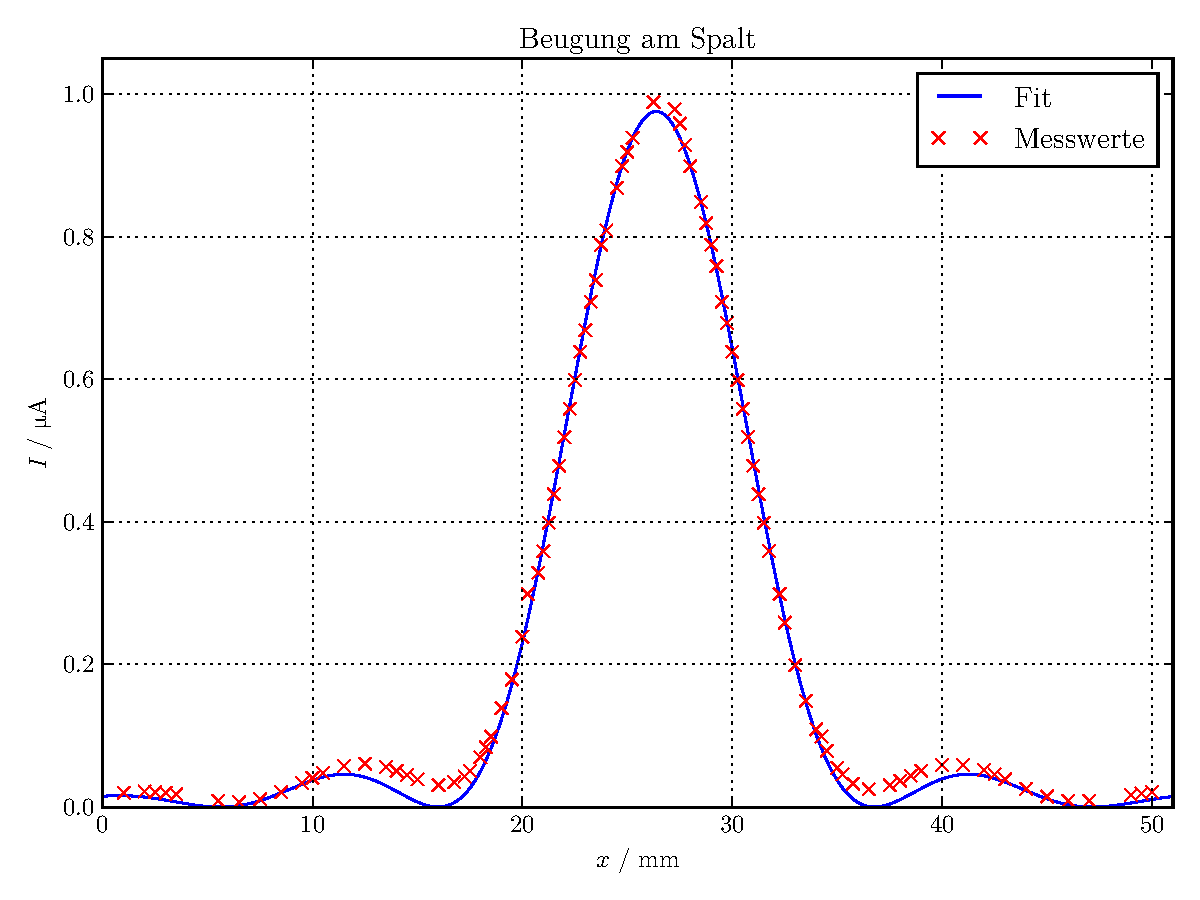
\includegraphics[width=\textwidth]{Plot.pdf}
  \caption{Graph der Messwerte und der Ausgleichsfunktion (Einzelspalt).}
  \label{fig:plot1}
\end{figure}
\subsection{Intensitätsverteilung am ersten Doppelspalt}
Bei der Messung am ersten Doppelspalt werden die in Tabelle \ref{tab:messwerte2}
stehenden Werte gemessen. Von diesen Werten wird zuerst der Dunkelstrom
$A_{d2}$ abgezogen und danach wie für den Einzelspalt mit Python ein Fit
an Formel \eqref{eqn:intensitätsverteilungdoppel} durchgeführt. Der Laser
und der Abstand zwischen Spalt und Photodiode bleiben unverändert. Als
Parameter ergeben sich:
\begin{align*}
  A_0 &= \SI{2.3(1)}{\micro\ampere}\\
  b &= \SI{100(6)}{\micro\meter}\\
  x_0 &= \SI{27.06(2)}{\milli\meter}\\
  s &= \SI{486(5)}{\micro\meter}
\end{align*}
Die Messwerte und die Ausgleichsfunktion sind in Abbildung \ref{fig:plot2}
dargestellt.
\begin{table}
  \centering
  \caption{Gemessener Diodenstrom bei der jeweiligen Position der Photodiode (ohne Abzug des Dunkelstroms).}
  \label{tab:messwerte2}
  \sisetup{table-format=2.2}
  \begin{tabular}{S S[table-format=4.0] | S S[table-format=4.0]}
    \toprule
     {$x$ in $\si{\milli\meter}$} & {$I$ in $\si{\nano\ampere}$} & {$x$} & {$I$} \\
    \midrule
    26.25 &  810 & 38.25 &  110 \\
    26.75 & 1680 & 39.25 &   52 \\
    27.25 & 1800 & 39.75 &   68 \\
    27.75 &  800 & 40.25 &   38 \\
    28.25 & 1300 & 25.75 & 1600 \\
    28.75 & 1650 & 25.25 & 1600 \\
    29.25 &  740 & 24.75 &  670 \\
    29.50 &  560 & 24.25 &  940 \\
    30.00 & 1000 & 23.75 & 1100 \\
    30.25 & 1100 & 23.25 &  440 \\
    30.75 &  520 & 23.00 &  300 \\
    31.25 &  320 & 22.50 &  500 \\
    31.50 &  420 & 22.25 &  530 \\
    31.75 &  480 & 21.75 &  240 \\
    32.25 &  260 & 21.25 &  100 \\
    32.75 &  110 & 21.00 &  130 \\
    33.25 &  120 & 20.75 &  140 \\
    33.75 &   69 & 20.25 &   73 \\
    34.25 &   45 & 19.75 &   27 \\
    35.00 &   56 & 19.25 &   45 \\
    35.75 &   40 & 18.75 &   37 \\
    36.25 &   94 & 18.25 &   33 \\
    36.75 &   90 & 17.75 &   84 \\
    37.25 &   48 & 17.25 &   87 \\
    37.75 &   90 & 16.75 &   48 \\
    38.25 &  110 & 16.25 &  100 \\
    39.25 &   52 & 15.75 &  110 \\
    39.75 &   68 & 15.25 &   50 \\
    \bottomrule
  \end{tabular}
\end{table}
\clearpage
\begin{figure}
  \centering
  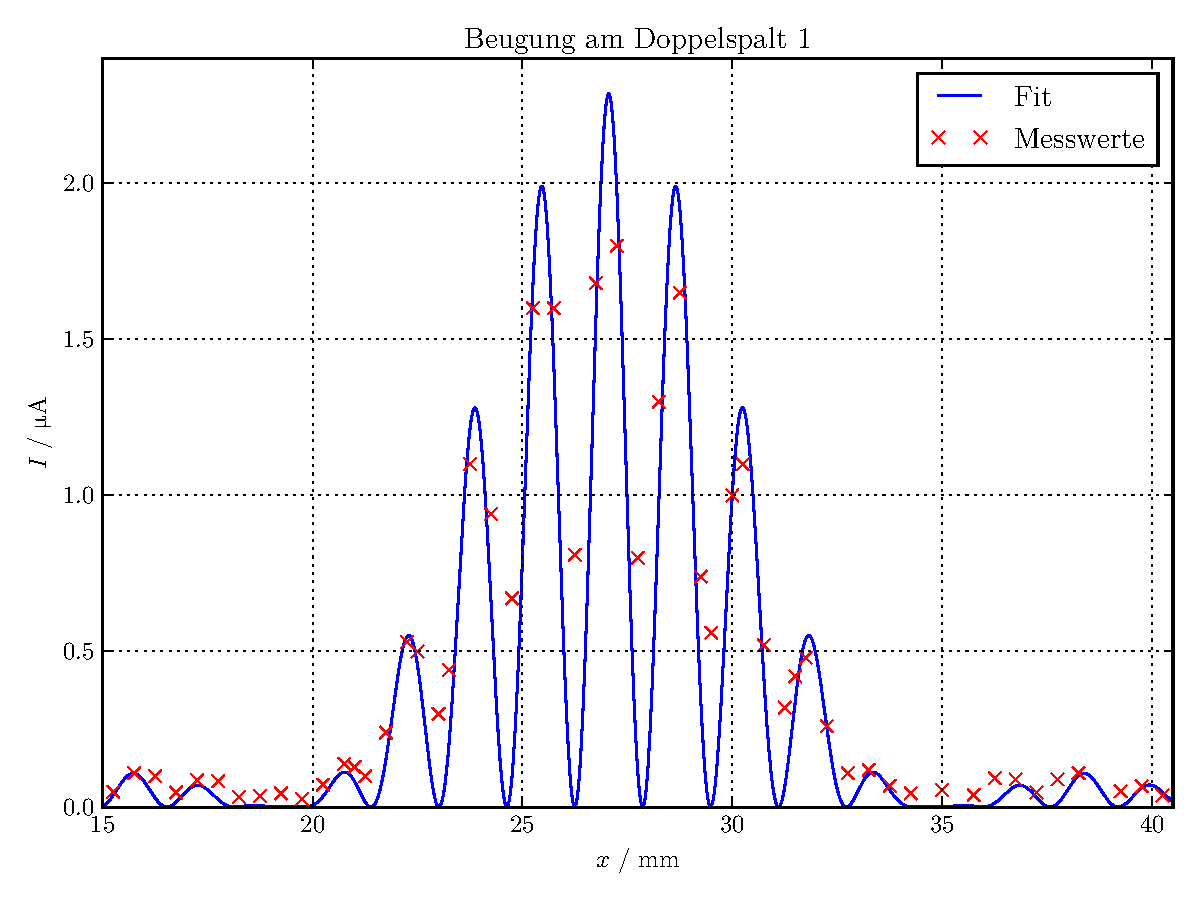
\includegraphics[width=\textwidth]{Plot2.pdf}
  \caption{Graph der Messwerte und der Ausgleichsfunktion (Doppelspalt Nr.1).}
  \label{fig:plot2}
\end{figure}
\subsection{Intensitätsverteilung am zweiten Doppelspalt}
Beim zweiten Doppelspalt werden die in Tabelle \ref{tab:messwerte3} stehenden
Werte gemessen. Erneut wird von diesen zuerst der Dunkelstrom $A_{d2}$
abgezogen. Mit der Anpassung an Formel \eqref{eqn:intensitätsverteilungdoppel}
ergeben sich bei gleichem Laser und gleichem Abstand die folgenden Parameter:
\begin{align*}
  A_0 &= \SI{2.98(7)}{\micro\ampere}\\
  b &= \SI{152(3)}{\micro\meter}\\
  x_0 &= \SI{27.62(2)}{\milli\meter}\\
  s &= \SI{238(3)}{\micro\meter}
\end{align*}
Die Messwerte und die Ausgleichsfunktion sind in Abbildung \ref{fig:plot3}
dargestellt.
\begin{table}
  \centering
  \caption{Gemessener Diodenstrom bei der jeweiligen Position der Photodiode (ohne Abzug des Dunkelstroms).}
  \label{tab:messwerte3}
  \sisetup{table-format=2.2}
  \begin{tabular}{S S[table-format=4.0] | S S[table-format=3.1]}
    \toprule
     {$x$ in $\si{\milli\meter}$} & {$I$ in $\si{\nano\ampere}$} & {$x$} & {$I$} \\
    \midrule
    26.25 &  500 & 25.75 &  360  \\
    26.75 & 1400 & 25.25 &  700  \\
    27.25 & 2500 & 24.75 &  800  \\
    27.75 & 2800 & 24.25 &  500  \\
    28.25 & 2000 & 23.75 &  210  \\
    28.75 &  800 & 23.25 &   44  \\
    29.25 &  290 & 22.75 &   12  \\
    29.75 &  520 & 22.25 &   21  \\
    30.25 &  780 & 21.75 &   60  \\
    30.75 &  670 & 21.25 &  110  \\
    31.25 &  350 & 20.75 &  110  \\
    31.75 &  100 & 20.25 &   62  \\
    32.25 &   32 & 19.75 &   28  \\
    32.75 &   30 & 19.25 &   29  \\
    33.25 &   64 & 18.75 &   37  \\
    33.75 &  120 & 18.25 &   30  \\
    34.25 &  140 & 17.75 &   20  \\
    34.75 &  100 & 17.25 &   11  \\
    35.25 &   42 & 16.75 &    8  \\
    35.75 &   16 & 16.25 &   18  \\
    36.75 &   32 & 15.25 &   52  \\
    37.75 &   19 & 14.25 &   26  \\
    38.75 &   14 & 13.25 &    7.4 \\
    39.75 &   48 & 12.25 &   13  \\
    40.75 &   44 & 11.25 &   18  \\
    \bottomrule
  \end{tabular}
\end{table}
\clearpage
\begin{figure}
  \centering
  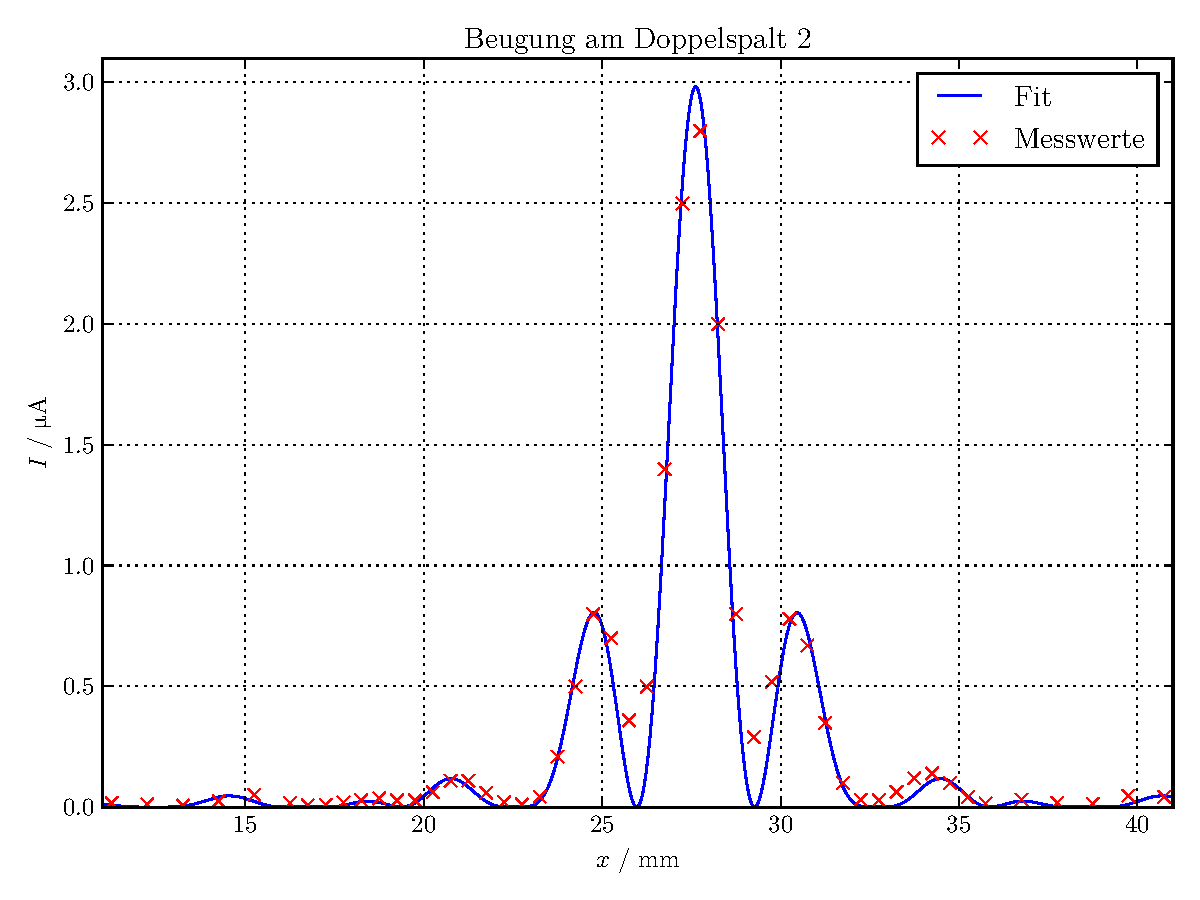
\includegraphics[width=\textwidth]{Plot3.pdf}
  \caption{Graph der Messwerte und der Ausgleichsfunktion (Doppelspalt Nr.2).}
  \label{fig:plot3}
\end{figure}
\subsection{Vergleich von Einzel- und Doppelspalt}
Für den Vergleich von Einzel- und Doppelspalt wird, unter Verwendung der
gleichen Parameter $b$ und $x_0$ mit Formel
\eqref{eqn:intensitätsverteilungeinzel} und eines angepassten Wertes der
Maximalintensität, die theoretische Kurve eines entsprechenden Einzelspalts
in den Graphen des ersten Doppelspalts aufgetragen.
Das Ergebniss ist in Abbildung \ref{fig:plot4} dargestellt.
\begin{figure}
  \centering
  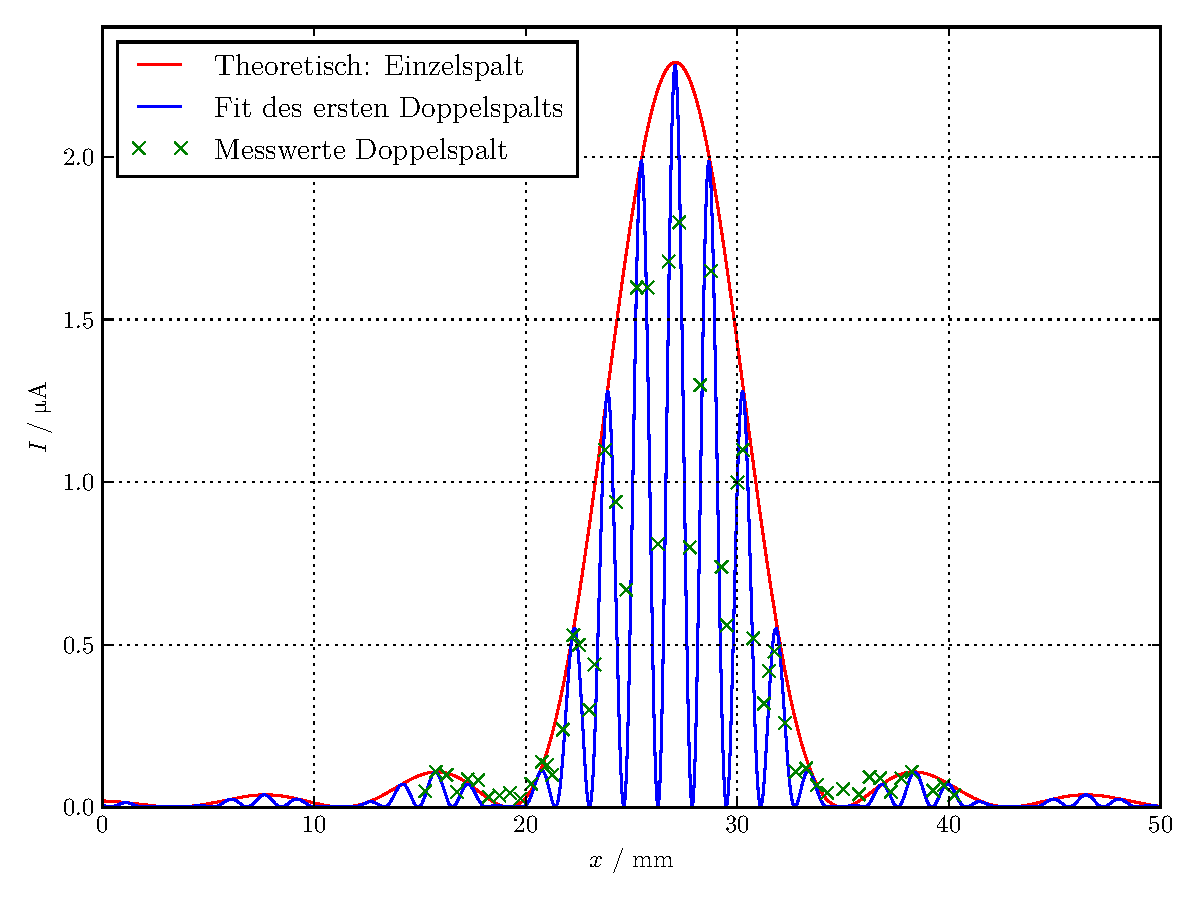
\includegraphics[width=\textwidth]{Plot4.pdf}
  \caption{Graph der Messwerte und der Ausgleichsfunktion (Doppelspalt Nr.1) und theoretischer Verlauf eines entsprechenden Einzelspalts.}
  \label{fig:plot4}
\end{figure}
\section{Diskussion}
\label{sec:diskussion}
Bei dem Versuch ergeben sich folgende Ergebnisse:
\begin{table}
  \centering
  \caption{Gemessener Diodenstrom bei der jeweiligen Position der Photodiode (ohne Abzug des Dunkelstroms).}
  \label{tab:messwerte1}
  \sisetup{table-format=3.1}
  \begin{tabular}{S S[table-format=3.0] S[table-format=2.1]}
    \toprule
    {Gemessen:} & {Herstellerangeben:} & {Abweichung in $\si{\percent}$} \\
    \midrule
    \text{$b_\mathup{E}$} = \SI{75.7(3)}{\micro\meter} & \text{$b_\mathup{E}$} = \SI{75}{\micro\meter} & 0.9\\
    \text{$b_\mathup{D1}$} = \SI{100(6)}{\micro\meter} & \text{$b_\mathup{D1}$} = \SI{100}{\micro\meter} & 0.0\\
    \text{$s_\mathup{D1}$} = \SI{486(5)}{\micro\meter} & \text{$s_\mathup{D1}$} = \SI{400}{\micro\meter} & 21.5\\
    \text{$b_\mathup{D2}$} = \SI{152(3)}{\micro\meter} & \text{$b_\mathup{D2}$} = \SI{150}{\micro\meter} & 1.3\\
    \text{$s_\mathup{D2}$} = \SI{238(3)}{\micro\meter} & \text{$s_\mathup{D2}$} = \SI{250}{\micro\meter} & 4.8\\
    \bottomrule
  \end{tabular}
\end{table}\\
Insgesamt liegen die gemessenen Spaltbreiten und Gitterkonstanten sehr nah an
den Herstellerangaben. Lediglich die Gitterkonstante beim ersten Doppelspalt
weicht etwas stärker davon ab. Mit dem Aufbau lassen sich also gut die Maße
von Spalten und Gittern bestimmen. Dabei ist das Ergebnis genauer, wenn der
Spalt sehr schmal ist, da das Beugungsmuster dann breiter und leichter
abtastbar ist.

\noindent
Beim Vergleich von Einzel- und Doppelspalt ist gut zu sehen,
dass der Verlauf des Einzelspalts die Einhüllende der Amplituden des
Doppelspalts darstellt. Außerdem ist beim Vergleich der beiden Doppelspalten
gut zu erkennen, dass die maximale Intensität mit einer größeren Spaltbreite
größer wird. Sie ist zudem doppelt so groß, wie die eines entsprechenden
Einzelspalts, da sich die Intensitäten der beiden Spalten am Doppelspalt
addieren. Die Einhüllende der Maxima wird mit größerer Spaltbreite schmaler,
was dem Verhalten des Beugungsmusters des Einzelspalts entspricht.
Eine größere Gitterkonstante sorgt dafür, dass zwischen den Maxima ein kleinerer
Abstand liegt und somit mehr Maxima in ein Maximum der Einhüllenden passen.
\nocite{*}
\printbibliography
\end{document}
